\documentclass[10pt,a4paper]{article}
\usepackage[margin=2cm]{geometry}
\usepackage{amsmath,amssymb,booktabs,graphicx,caption,subcaption,xcolor,float,hyperref,tikz}
\usetikzlibrary{arrows.meta,positioning,calc}
\hypersetup{colorlinks=true,linkcolor=blue!50!black,urlcolor=blue!50!black}
\captionsetup{font=small,labelfont=bf}
\newcounter{diagram}
\newcommand{\diagramcaption}[1]{\refstepcounter{diagram}\par\smallskip\noindent{\small\textbf{Diagram~\thediagram.} #1}}
\title{\vspace{-1.2cm}\textbf{Saying less, steering more}\\[2pt]
\large Simulation 2 (asynchronous activation), setup \texttt{task003-nosolution}: first results}
\author{LLM-free simulator, runs of 9 October 2026}
\date{}
\begin{document}
\maketitle
\vspace{-1cm}

\paragraph{Summary.} 24 agents hold evidence that, pooled, is a coin flip between allocation
A0 (the truth) and A2, with no proof available to anyone. Simulation 2 removes the day/night
rounds of Simulation 1: agents and the controller act at random times, remembered facts fade
continuously, and the shared board fades too. Both controllers still tip the swarm, and
\textbf{the effect persists} after they stop. When agents forget, control is
\textbf{weaker than in Simulation 1} (truth $0.29$ against $0.42$; false $0.19$ against
$0.28$); with full memory it is the same. The controller's rate barely matters when agents
forget. With full memory, \textbf{a faster controller steers less}: it puts more of its pool
into circulation, and the whole pool pulls every belief toward the same point whatever the
target. Turning the vote gate off adds about 16 messages per episode and no control.
Main hypotheses were confirmed on a second, independent set of random draws.

\section{Setup}

\begin{center}
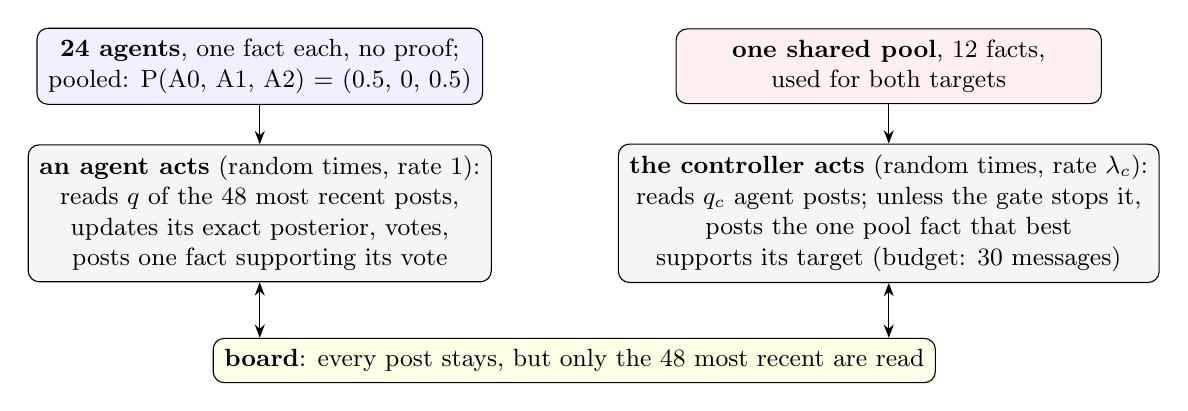
\begin{tikzpicture}[font=\small, box/.style={draw, rounded corners, align=center, inner sep=4pt}]
  \node[box, fill=gray!8, minimum width=5.4cm] (agent) {\textbf{an agent acts} (random times, rate 1):\\
     reads $q$ of the 48 most recent posts,\\ updates its exact posterior, votes,\\ posts one fact supporting its vote};
  \node[box, fill=gray!8, right=1.6cm of agent, minimum width=5.4cm] (ctrl) {\textbf{the controller acts} (random times, rate $\lambda_c$):\\
     reads $q_c$ agent posts; unless the gate stops it,\\ posts the one pool fact that best\\ supports its target (budget: 30 messages)};
  \node[box, fill=blue!6, above=0.5cm of agent, minimum width=5.4cm] (agents) {\textbf{24 agents}, one fact each, no proof;\\
     pooled: P(A0, A1, A2) = (0.5, 0, 0.5)};
  \node[box, fill=red!6, above=0.5cm of ctrl, minimum width=5.4cm] (pool) {\textbf{one shared pool}, 12 facts,\\
     used for both targets};
  \coordinate (mid) at ($(agent.south)!0.5!(ctrl.south)$);
  \node[box, fill=yellow!10, anchor=north, minimum width=8cm] (board) at ($(mid)+(0,-0.7)$) {\textbf{board}: every post stays, but only the 48 most recent are read};
  \draw[-{Stealth}] (agents) -- (agent);
  \draw[-{Stealth}] (pool) -- (ctrl);
  \draw[{Stealth}-{Stealth}] (agent.south) -- (agent.south |- board.north);
  \draw[{Stealth}-{Stealth}] (ctrl.south) -- (ctrl.south |- board.north);
\end{tikzpicture}
\diagramcaption{Simulation 2. There are no rounds. Each remembered fact is forgotten after a
random lifetime (on average a fraction $\rho$ survives one time unit) and comes back if read
again. The controller acts for $0 \le t < 30$; agents continue alone until $t = 40$.}
\end{center}

\noindent The agents' facts plus the \emph{whole} pool give P(A0, A1, A2) = (0.75, 0, 0.25):
the truth keeps an edge that cannot be designed away, because every fact is true. Agents are
exact Bayesian reasoners and vote by probability matching (the vote is drawn from the
posterior). The \emph{vote gate} keeps the controller silent when at least 75\% of the posts
it read come from agents who voted for its target. The grid: posts read $q \in \{3,6,12\}$,
$q_c \in \{3,6,12,24\}$, memory $\rho \in \{0.75, 1\}$, controller rate
$\lambda_c \in \{0.5,1,2,4,8\}$ actions per time unit, gate on/off; 1{,}000 episodes per
setting. Control is measured by the \emph{gain}
\begin{equation}\label{eq:gain}
G(t) = \frac{1}{E}\sum_{e=1}^{E}\Bigl[m_{\text{target}}(t)^{\text{ctrl}}(e) - m_{\text{target}}(t)^{\text{silent}}(e)\Bigr],
\end{equation}
where $m_k(t)$ is the agents' mean belief in allocation $k$ and each episode $e$ uses the same
random draws with and without the controller. Unless stated otherwise: $q = 6$, $q_c = 12$,
gate on.

\section{Main result: both controllers tip the swarm, and the effect stays}

\begin{table}[H]
\centering\small
\caption{Gain at $t = 30$, Eq.~(\ref{eq:gain}), $\lambda_c = 1$, gate on; in brackets the
silent swarm's belief in the target. Simulation 1: one fact per night, same $q$, $q_c$, $\rho$.}
\label{tab:main}
\begin{tabular}{llccc}
\toprule
$\rho$ & controller & Simulation 2 & Simulation 1 & messages sent \\
\midrule
0.75 & truth (A0) & 0.29 (0.38) & 0.42 & 11 \\
0.75 & false (A2) & 0.19 (0.48) & 0.28 & 12 \\
1 & truth (A0) & 0.38 (0.50) & 0.38 & 7 \\
1 & false (A2) & 0.14 (0.50) & 0.15 & 15 \\
\bottomrule
\end{tabular}
\end{table}

\begin{figure}[H]
\centering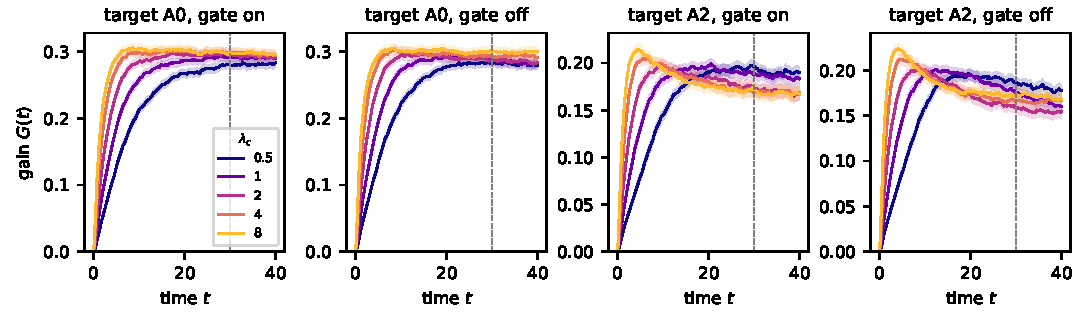
\includegraphics[width=0.98\linewidth]{figures/fig_gain_time.pdf}
\caption{Gain over time by controller rate $\lambda_c$, $\rho = 0.75$; the controller stops at
$t = 30$ (dashed). Bands: 95\% intervals.}
\label{fig:gaintime}
\end{figure}

\begin{itemize}\itemsep1pt
\item \textbf{Both controllers tip the swarm} (Table~\ref{tab:main}); the truth controller is
  stronger, as in Simulation 1.
\item \textbf{When agents forget, control is weaker than in Simulation 1}, by $0.14$ (truth) and
  $0.09$ (false) with fresh random draws. With full memory the two simulations agree within
  $0.01$. In Simulation 1 memories change only at dawn and every agent acts right after a full
  day of posts; here facts expire at random moments between actions, so fewer of the
  controller's facts are held together at any time.
\item \textbf{The effect persists}: ten time units after the controller stops, the gain has
  changed by at most $0.016$ at $\rho = 0.75$ (Figure~\ref{fig:gaintime}); agents keep
  relaying the controller's facts (12--45\% of their posts).
\end{itemize}

\begin{figure}[H]
\centering
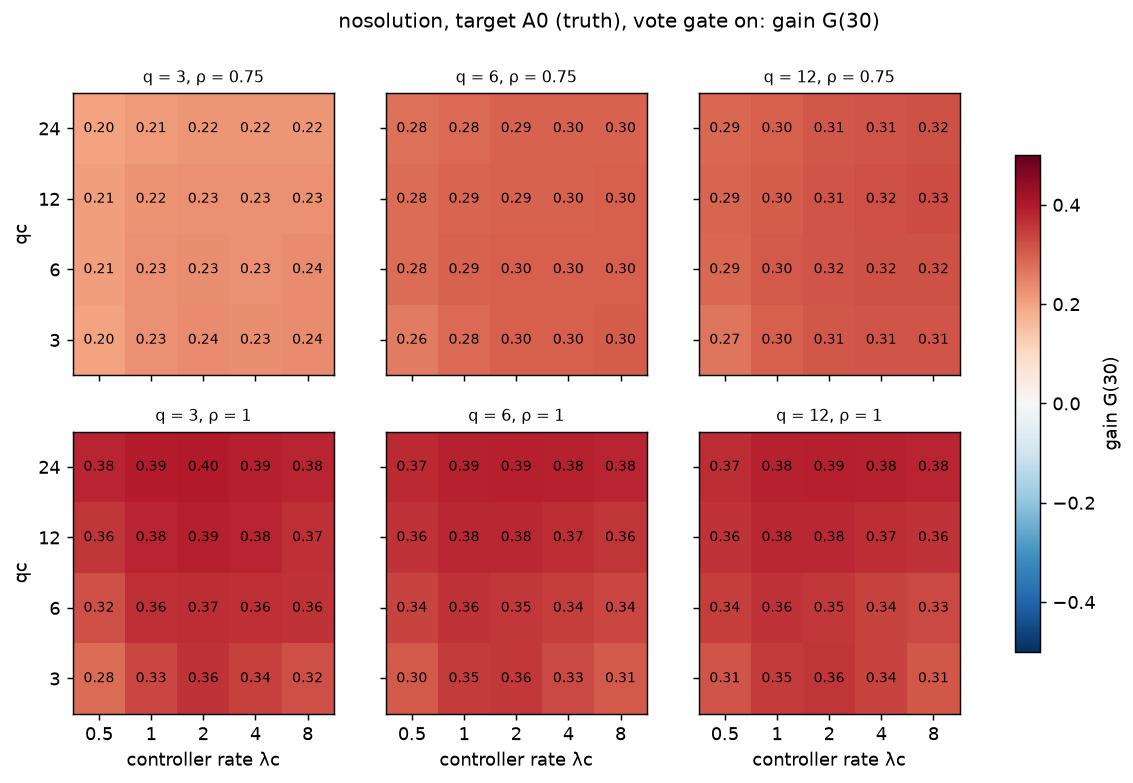
\includegraphics[width=0.72\linewidth]{figures/phase_truth_gateon.png}\\[2pt]
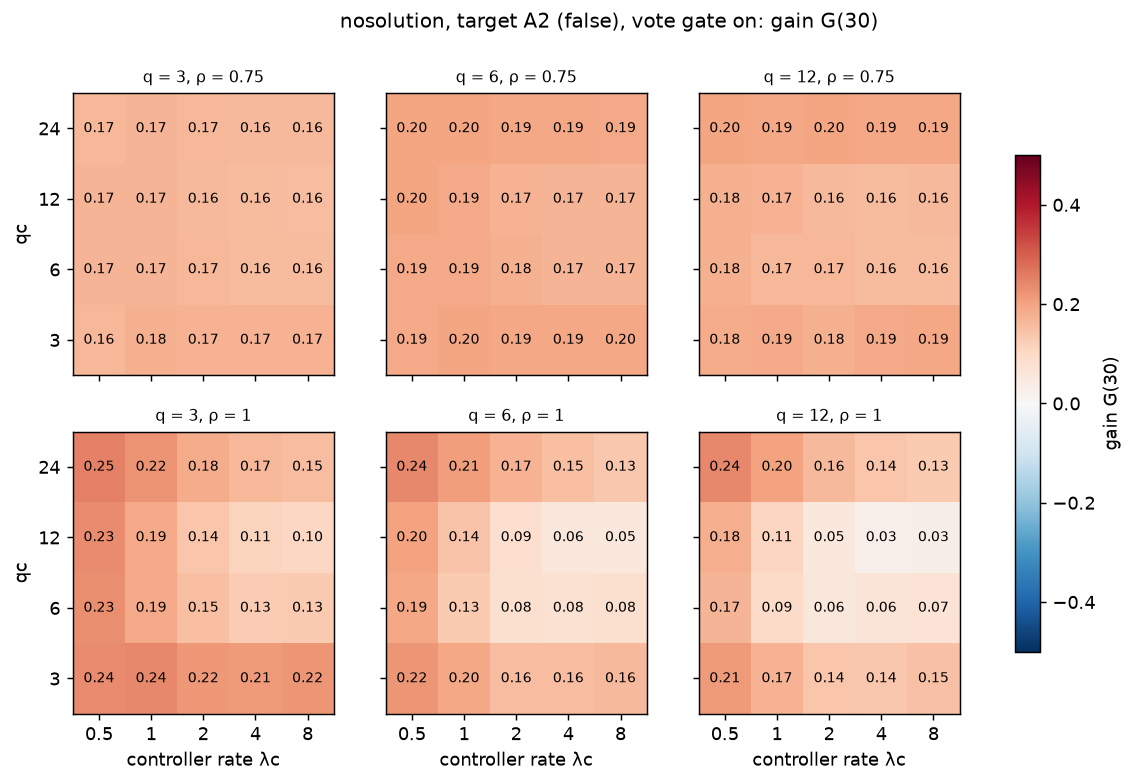
\includegraphics[width=0.72\linewidth]{figures/phase_false_gateon.png}
\caption{Gain $G(30)$ over controller rate (x) and posts read by the controller $q_c$ (y), for
every $q$ (columns) and $\rho$ (rows); gate on. Top: target A0; bottom: target A2.}
\label{fig:phase}
\end{figure}

\section{The controller's rate}

\begin{figure}[H]
\centering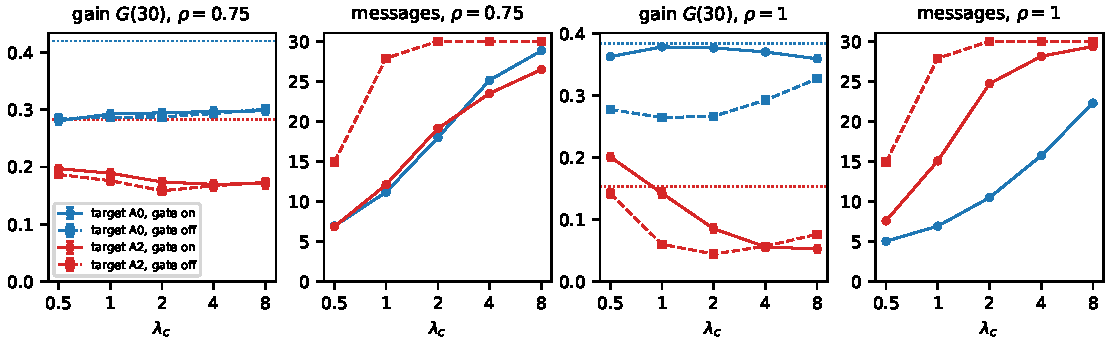
\includegraphics[width=0.98\linewidth]{figures/fig_rate.pdf}
\caption{Gain at $t = 30$ and messages sent against the controller rate, for $\rho = 0.75$
and $\rho = 1$ (target A0 blue, A2 red; gate on solid, off dashed; dotted: Simulation 1).}
\label{fig:rate}
\end{figure}

\paragraph{When agents forget, the rate barely matters.} From $\lambda_c = 0.5$ to $8$ the gain
moves from $0.28$ to $0.30$ (truth) and from $0.20$ to $0.17$ (false), but the messages sent
rise from about 7 to 26--29. A fast controller spends its budget early (by $t \approx 4$ with
the gate off), reaches its gain sooner, and then the gain stays put. Gain per message is
highest for a slow, gated controller.

\paragraph{With full memory, a faster controller steers less.} The false controller's gain
falls from $0.20$ at $\lambda_c = 0.5$ to $0.05$ at $\lambda_c = 8$, and with the gate off the truth controller
loses $0.05$ on average against the gate on, up to $0.12$ (Figure~\ref{fig:rate}, right). The
same fall appears at every $q$ and at $q_c$ = 3, 6 and 12 (Figure~\ref{fig:phase}, bottom rows).

\begin{figure}[H]
\centering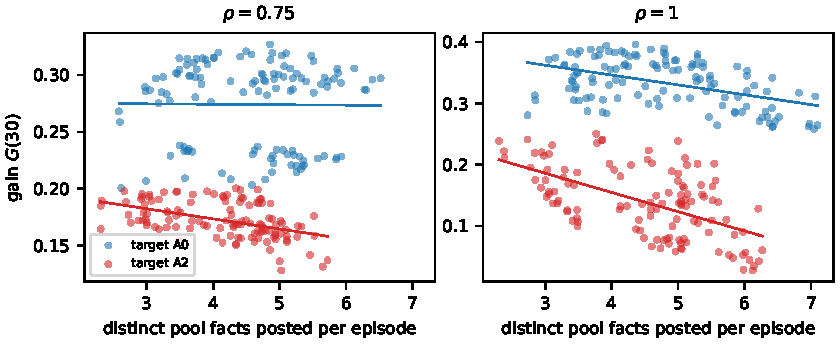
\includegraphics[width=0.66\linewidth]{figures/fig_distinct.pdf}
\caption{Each point is one setting ($q$, $q_c$, $\lambda_c$, gate): gain at $t = 30$ against the
number of different pool facts the controller posted per episode. Lines: least-squares fits.}
\label{fig:distinct}
\end{figure}

\noindent\textbf{Why: saying more of the pool pulls toward the same point.} Every fact is true,
and the agents' facts plus the whole pool give (0.75, 0, 0.25). With full memory nothing posted
is forgotten, so the more \emph{different} pool facts a controller puts into circulation, the
closer beliefs move to that point, whatever its target: down from the false controller's
side, and down from the truth controller's best, which lies above 0.75. At $\rho = 1$ each
additional distinct fact lowers the gain by $0.031$ (false) and $0.016$ (truth)
(Figure~\ref{fig:distinct}, right). The rate sets that number: spread over 30 time units, the
controller reads varied boards and posts more different facts (6.3 per episode at
$\lambda_c = 1$, gate off); at $\lambda_c = 8$ it spends its budget in a burst on similar boards
and repeats itself (5.0), which is why the gain partly recovers there. When agents forget,
facts leave again and the effect is weak (Figure~\ref{fig:distinct}, left). This was found
after looking at the data, so it was rerun with fresh random draws: \textbf{every one of the 16 checked reversals
reappeared} (false controller, gain at $\lambda_c = 0.5 \ldots 8$: 0.20, 0.15, 0.08, 0.05,
0.05). The explanation by distinct facts rests on a correlation across settings and is not yet
tested directly (for example with a controller that remembers what it has said).

\section{The vote gate}

The gate keeps the controller silent when it reads enough support. Turning it off adds about
16 messages per episode at $\lambda_c = 1$ (confirmed with fresh draws) and \textbf{no control} when agents
forget ($-0.017$ and $-0.003$); with full memory it \emph{lowers} the gain (truth $-0.05$ on
average) through the mechanism above.

\section{The controller overestimates its support}

\begin{figure}[H]
\centering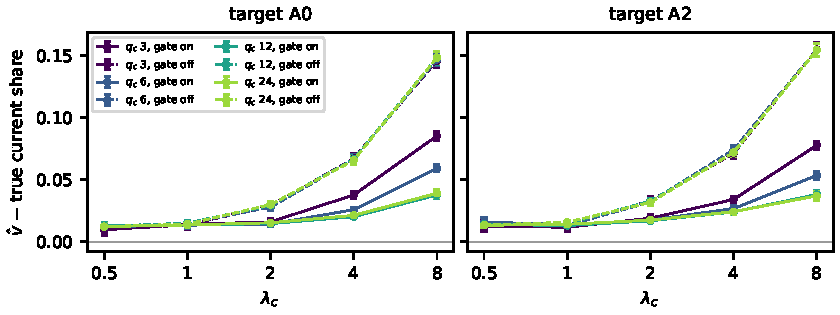
\includegraphics[width=0.66\linewidth]{figures/fig_sensing.pdf}
\caption{Error of the controller's estimate $\hat v$ (share of posts read whose author voted
for the target) against the true current share of all 24 agents' last votes; $\rho = 0.75$;
solid gate on, dashed off.}
\label{fig:sensing}
\end{figure}

Unlike in Simulation 1, $\hat v$ is biased upward, and \textbf{the faster the controller, the
larger the bias}: about $+0.014$ at $\lambda_c \le 1$, rising to $+0.05$ (gate on) and $+0.15$
(gate off) at $\lambda_c = 8$. A likely reason, not yet tested: the posts it reads come from agents who
acted recently, often just after reading the controller's facts, while the true share also
counts older votes. More posts read ($q_c$) reduce the error's spread (0.16 at $q_c = 3$, 0.07
at $q_c = 24$) but not the bias.

\paragraph{Caveats.} One world (task\_003), 24 agents, exact-Bayesian agents,
probability-matching votes; a controller without memory that posts one fact at a time; a
budget of 30 messages. Means over 1{,}000 episodes per setting. Full analysis, code and
tables: \texttt{analysis/task003\_llm\_free/simulation\_2/analysis/} (report of 9 October,
reviewer guide).

\end{document}
